\documentclass{report}
\usepackage[utf8]{inputenc}
\usepackage[top=2.5cm, left=2.3cm, right=2.7cm, bottom=3.0cm]{geometry}
\usepackage{float}
\usepackage{hyperref}
\usepackage{pdfpages}
\usepackage{sectsty}
\usepackage{titlesec}
\usepackage{listings}
\setcounter{secnumdepth}{4}
\titleformat{\paragraph}
{\normalfont\normalsize\bfseries}{\theparagraph}{1em}{}
\titlespacing*{\paragraph}
{0pt}{3.25ex plus 1ex minus .2ex}{1.5ex plus .2ex}



\titleformat{\chapter}{\normalfont\huge}{\thechapter.}{20pt}{\huge}
\newcommand{\ubar}[1]{\underaccent{\bar}{#1}}
\newcommand{\e}[1]{\cdot10^{#1}}


\title{Main Coursework \\ Computational Intelligence \\ COMP-575}
\author{Tudor Jianu [201532511]}
\date{13-05-2021}
\usepackage{graphicx}
\usepackage{amsmath}
\begin{document}
\lstset{language=Python} 

\maketitle

\chapter{Perceptron}

   The Perceptron is a simple error correction algorithm that aims at fitting a line called decision boundary that separates the given classes. The Perceptron is able to learn by correcting its output through the adjustment of weights such that the output equals the target. 
Generally, the weights of the Perceptron are initialised to zero although this implementation made use of the NumPy random library and generated a set of weights in the $(0,1]$ interval while the learning rate $\eta$ has been made available to the user to select it. The activation function implemented has been a simple sign function that maps the values of $z=W(t)^{T} x(t)$ based on the sign of the output such as:

\begin{center}
$\begin{cases}
    1 & \text{, if } x > 0\\
    -1 & \text{, if } x \leq 1\\
\end{cases}$
\end{center}

The adaptation of the Perceptron to the error takes place by subtracting from the real output, the predicted output. This means that in the case of matching labels, the subtraction will equal $0$ meaning that no update is going to take place. In the case of difference, the subtraction will equal $2$ and $-2$ respectively which result is then multiplied by the input vector $X$ and the learning rate $\eta$. In more concrete terms, the update rule simply shifts the decision boundary such as if the sign is negative, the algorithm distances the decision boundary from the data point whereas if the sign is positive, it closes the distance. In mathematical form the above update rule is presented as following:

\begin{center}
$ W(t+1) = W(t) + \eta [d(t) - y(t)] * x(t)
$
\end{center}

In order to correctly predict the classes, the data target feature has been set to be a +1 for one class and -1 for the other class. This can be more generalised and predict the target class while making the rest of the classes -1. 
The process described above continues iteratively, taking one instance at a time, until a number of iterations is reached or until the algorithm converges. In the case of convergence, if the data is not linearly separable, the decision boundary will continue to be shifted thus making the convergence impossible.

Bellow, the decision boundary traced by the Perceptron algorithm can be observed. The Perceptron has been trained on randomly generated data using a learning rate of $\eta=0.1$ and the number of iterations $n\_iter=4$. The cluster labels have been changed to 1 and -1 respectively. From the first graph, it can be seen that as long as the data takes the form of two distinguishable clusters, the algorithm has no issues to separate the two, achieving an accuracy of 98\%, whilst, in the second graph, it can be seen that although the algorithm managed to draw a reasonable boundary, achieving 79\%, it is still constrained by the fact that is linear and cannot comprehend more complex shapes. 


\begin{figure}[htp]
\centering
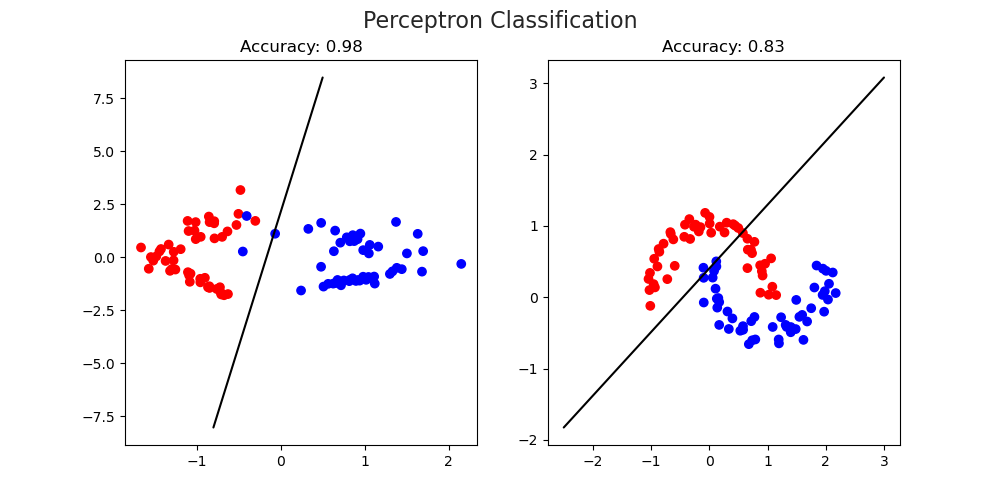
\includegraphics[scale=0.70]{Perceptron/Graphs/Perceptron.png}
\caption{Perceptron}
\label{Perceptron}
\end{figure}



\chapter{Multi-Layer Perceptron}

The Multi-Layer Perceptron (MLP) differs from the classical Perceptron in terms of the layers of neurons that compose it. By having more layers combined with non linear activation functions, the MLP is capable of classifying more complex data such as the moons from the previous Perceptron example. 

\section{Introduction to MLP}

\subsection{Forward Pass}
Similarly to the Perceptron, the algorithm takes an object $X$ of $n$ features and computes $z^{(L)}=X\cdot W^T+b$. The result is then passed through an activation function such as the sigmoid activation giving $a^{(L)}=\sigma(z^{(L)})$. This process is repeated for all of the layers until the final output layer. The output layer differs in relation to the hidden layers by not having a bias term included. The output correctness is measured through a cost function such as Mean Squared Error which takes the output of the MLP and compares it with the true value through the following formula:

\begin{center}
$MSE = (a^{(L)}-y)^2$
\\
Where, $a^{(L)} = \text{MLP output}$ and $y = \text{true label}$
\end{center}

\begin{figure}[htp]
\centering
\includegraphics[scale=0.40]{MLP/Graphs/Backpropag.png}
\caption{Basic Flow of MLP}
\label{Backpropagation}
\end{figure}
\break
\subsection{Backward Pass}


After the cost has been computed, the algorithm uses the derivative of the cost function in combination with the chain rule in order to find the degree of change in cost influenced by each weights. As such, the algorithm uses the chain rule to propagate backward the error, hence the name. In the first phase, the error in $z$ is calculated for all of the layers. The output layer's error in $z$, is calculated by using the fact that:

\begin{center}
$\frac{\partial C_0}{\partial z^{(L)}} = \frac{\partial C_0}{\partial a^{(L)}}\cdot \frac{\partial a^{(L)}}{\partial z^{(L)}} = \delta^{(L)}$
\end{center}


,from which $\frac{\partial C_0}{\partial a^{(L)}}$ is equal to: 
\begin{center}
$MSE'=2(a^{(L)}-y)$
\end{center}

And $\frac{\partial a^{(L)}}{\partial z^{(L)}}$ is given, in the case of sigmoid activation function, by:

\begin{center}
$ \sigma'(z^{(L)})$
\end{center}

, which results in:
\begin{center}
$ \delta^(L) = 2(a^{(L)}-y) \odot \sigma'(z^{(L)})$
\end{center}

In the case of the hidden layer, the error in $z$ is calculated in relation to $\delta^{(L)}$ using:

\begin{center}
$\frac{\partial z{(L)}}{\partial z^{(L-1)}} = \frac{\partial z^{(L)}}{\partial a^{(L-1)}}\cdot \frac{\partial a^{(L-1)}}{\partial z^{(L-1)}}$
\end{center}

Considering that $z = X\cdot W^T +b$ and by considering a sigmoid activation function, the formula transforms in:

\begin{center}
$ \delta^{(L)} \cdot W^T \odot \sigma'(z^{(L-1)})$
\end{center}

By having the error in $z$, now it can be propagated for each layer to the weights:
\begin{center}
$ \frac{\partial z{(L)}}{\partial W^{(L)}} = \delta^{(L)}\cdot a^{(L-1)}$
\end{center}

and to the biases:

\begin{center}
$ \frac{\partial z{(L)}}{\partial b^{(L)}} = \delta^{(L)}\cdot 1$
\end{center}


\subsection{Updating Phase}

After the error has been propagated to all of the weights and biases, the algorithm adapts its weights:

\begin{center}
$ W^{(L)}(t+1) = W^{(L)}(t) - \eta \cdot \delta^{(L)}\cdot a^{(L-1)}$
\end{center}

and bias:

\begin{center}
$ b^{(L)}(t+1) = b^{(L)}(t) - \eta \cdot \delta^{(L)}$
\end{center}

,thus completing one iteration.

There is just a slight change in the notation when it comes to the flow of the algorithm.

\section{In code}

The only requirement for implementing the code for the algorithm is NumPy.


\subsection{Activations}
The activation function takes the output of the layer and maps it to a non linear output. As such, the function contains one input ($z$) and one output $(a)$:

\lstinputlisting[language=Python, firstline=7, lastline=11]{MLP/Activations.py}

As there are multiple activation functions, in this report five were used and all inherited from the previous defined class, Activations. The first activation function implemented is the most basic Identity activation which does not alter the $z$:

\lstinputlisting[language=Python, firstline=30, lastline=38]{MLP/Activations.py}

When considering the backward propagation, the class can have a backward method that allows it to output the derivative of the activation in $z$. In the case of the simple Identity activation, the derivative is simply 1:

\lstinputlisting[language=Python, firstline=40, lastline=44]{MLP/Activations.py}

In a similar fashion each activation class is created. For example, the sigmoid activation ($\sigma(z)$) which scales the data into the interval $(0,1]$, has the same initialisation as the Identity one with an extra parameter $\alpha$ which controls the scale of the output:

\lstinputlisting[language=Python, firstline=14, lastline=23]{MLP/Activations.py}

and when it comes to the backward method, given that the derivative of the sigmoid function is $\sigma'(z)=\sigma(z)\cdot (1-\sigma(z))$ the method does not need to recompute $\sigma(z)$ which saves some computation time:


\lstinputlisting[language=Python, firstline=25, lastline=27]{MLP/Activations.py}

All of the other activation functions are registered in the same manner.

\subsection{Cost function}
The cost function is implemented similarly to the activation functions classes, holding two methods for both the forward and backward phase. In the forward phase, the cost gets outputted as the mean of all costs:

\lstinputlisting[language=Python, firstline=10, lastline=16]{MLP/Loss.py}

while in the backward phase, it returns the derivative:

\lstinputlisting[language=Python, firstline=18, lastline=26]{MLP/Loss.py}


\subsection{The Layer}

The layer class takes the activation and number of neurons and contains the biases ($B$), the weights ($W$),  the input ($x$ in case of the first layer and $a^{(L-1)}$ otherwise), and $z$, the result of $X\cdot W^{T} + b$.  The main parameters of each layer are its activation function and its number of neurons: 

\lstinputlisting[language=Python, firstline=8, lastline=16]{MLP/Layers.py}

Now that the layer class is created, it has to populate its weights and biases with the required matrices. In order to avoid transposing the weights every time a forward pass is done, the matrix is created in an already transposed form. This is done using NumPy's random module and the shape of the input data is passed as the number of rows, while the number of neurons is passed as the number of columns. The bias, is created in a similar fashion and in a transposed form so that it resembles the one bias/neuron shape. This method will be incorporated into the first forward pass as the algorithm only requires one random initialisation of the weights and biases.

\lstinputlisting[language=Python, firstline=21, lastline=23]{MLP/Layers.py}

Furthermore, the layer has to have the ability to update its weights based on the local error in $z$ which is done by:

\lstinputlisting[language=Python, firstline=25, lastline=30]{MLP/Layers.py}

There are two distinguishable layers, the Dense - hidden layer- and the Output layer. The Dense Layer contains two main methods, the forward method which saves the inputs, $z$, and $a$ and returns the output of the computations:

\lstinputlisting[language=Python, firstline=37, lastline=43]{MLP/Layers.py}

And a backward method which takes the upper error from the next layer and computes the error in $z$, returning this error so that in can be further propagated:

\lstinputlisting[language=Python, firstline=45, lastline=49]{MLP/Layers.py}

The output layer behaves in a similar manner but additionally, it does not have the bias term for updates while it's backpropagation starts by calculating the cost:

\lstinputlisting[language=Python, firstline=74, lastline=77]{MLP/Layers.py}

And propagates the error:

\lstinputlisting[language=Python, firstline=79, lastline=82]{MLP/Layers.py}


\subsection{The Model}

Having the activation, the layer, and the cost function, the model can emerge. Starting with the initialisation, the model contains the number of epochs it will iterate for, the seed (number to allow reproducible results), the batch size (amount of objects feed to the algorithm at one time), $\alpha$ (the learning rate), and $\mu$ (the momentum parameter). Besides, the model will contain the costs at each epoch, the layer objects and the averages of the costs:

\lstinputlisting[language=Python, firstline=9, lastline=20]{MLP/Model.py}

In order to add a layer to the model, a method needs to be created:

\lstinputlisting[language=Python, firstline=22, lastline=24]{MLP/Model.py}

Besides, the model needs a forward method that will take the input and pass it through each layer and compute the cost at the end:

\lstinputlisting[language=Python, firstline=47, lastline=52]{MLP/Model.py}

With the forward phase completed, the backward phase can begin. First the layers have to be reversed as the process starts with the Output layer first. Then the error is computed and gets passed to each layer and at the end, the order of the layers is restored:

\lstinputlisting[language=Python, firstline=55, lastline=60]{MLP/Model.py}

As each error of z is computed, the update phase can begin. This is implemented by:

\lstinputlisting[language=Python, firstline=63, lastline=66]{MLP/Model.py}

Those three phases are repeated for the number of epochs times and the cost is printed:

\lstinputlisting[language=Python, firstline=67, lastline=75]{MLP/Model.py}

Additionally, a prediction method is included which instead of computing the cost at the end of the forward phase, it computes the predicted value of each element:

\lstinputlisting[language=Python, firstline=36, lastline=44]{MLP/Model.py}

While the sampling method allows for the use of batches:

\lstinputlisting[language=Python, firstline=26, lastline=31]{MLP/Model.py}



\section{Comparing parameters}

\subsection{The Dataset}

The dataset used throughout the comparison is the Boston House Prices dataset, available from \href{https://scikit-learn.org/stable/modules/generated/sklearn.datasets.load_boston.html#sklearn.datasets.load_boston}{Scikit-Learn}. The dataset contains 506 instances and 13 features. All of the features are real, positive numbers while the target value (the house prices) is bounded by the interval $[5;50]$. All of the features have been normalised before feeding it into the model.

\newpage
\subsection{Learning Rate}
With everything else set to default, the activation functions performed as following: 

\subsubsection{Sigmoid}

In the case of the Sigmoid Activation Function, it can be seen that a learning rate of $\eta = 0.01$, the algorithm did not managed to converge to a solution. In the case of the other learning rates, under the same epoch constraints, the best average cost has been achieved by the learning rate of $\eta = 0.01$. It seems that neither a higher, nor a low learning rate is good for an architecture based on this activation function.
\begin{figure}[htp]
\centering
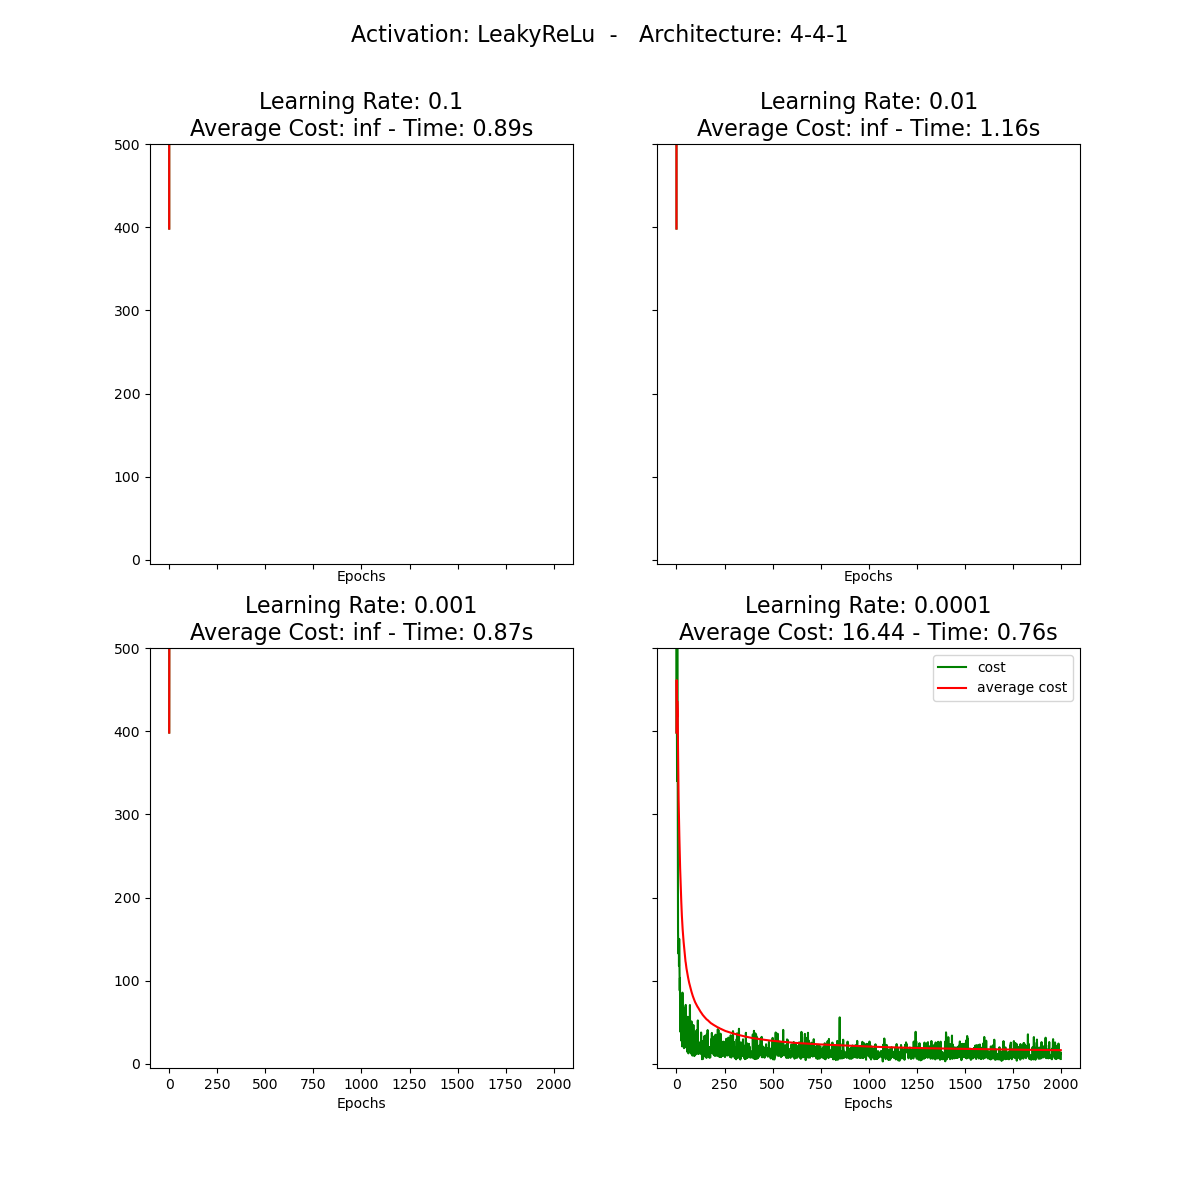
\includegraphics[scale=0.54]{MLP/Graphs/lrSigmoid.png}
\caption{Sigmoid: Learning Rate Differences}
\label{sigmoidLr}
\end{figure}

\newpage

\subsubsection{TanH}

In the case of the TanH activation function, it can be observed that the results are quite different. While both the learning rates of $\eta = 0.1$ and $\eta = 0.01$ have not been able to converge, a lower learning rate of $\eta = 0.0001$ seem to work better for this Activation function as it converged to a lower Average cost than the learning rate of $\eta= 0.001$.

\begin{center}
\begin{figure}[htp]
\includegraphics[scale=0.54]{MLP/Graphs/lrTanH.png}
\caption{TanH: Learning Rate Comparison}
\label{lrTanH}
\end{figure}
\end{center}

\newpage
\subsubsection{ReLu}

The Rectified Linear Unit (ReLu) activation function failed to converge when the learning rate was $\eta \geq 0.001$ while a learning rate of $\eta = 0.0001$, besides converging, it showed the lowest average cost of $16.25$.
\begin{center}
\begin{figure}[htp]
\includegraphics[scale=0.54]{MLP/Graphs/lrReLu.png}
\caption{ReLu: Learning Rate Comparison}
\label{lrTanH}
\end{figure}
\end{center}

\newpage
\subsection{LeakyReLu}
Leaky ReLu performed in a similar fashion to ReLu, achieving a similar kind of results with the only difference being that the algorithm diverged to infinity.

\begin{center}
\begin{figure}[htp]
\includegraphics[scale=0.54]{MLP/Graphs/lrLeakyReLu.png}
\caption{Leaky ReLu: Learning Rate Comparison}
\label{lrTanH}
\end{figure}
\end{center}

\newpage
\subsection{Number of Hidden Layers}

\subsubsection{Architecture: 4-1}
It can be visualised that the sigmoid was able to converge with an average score of $18.96$ whereas the others could not converge.
\begin{center}
\begin{figure}[htp]
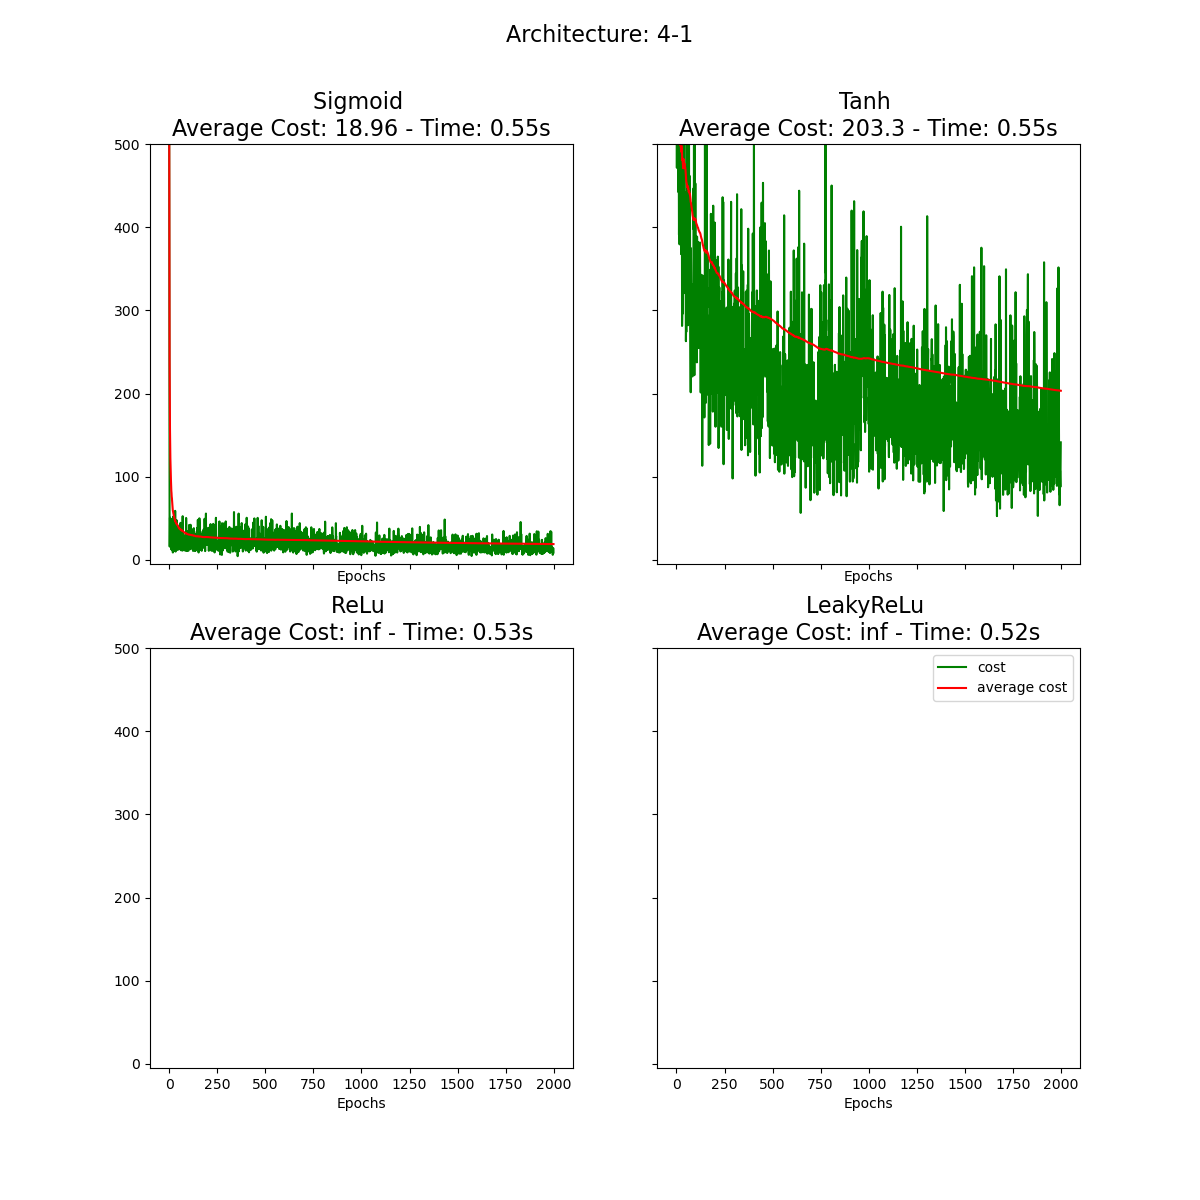
\includegraphics[scale=0.54]{MLP/Graphs/oneHidden.png}
\caption{Architecture Comparison 1}
\label{a41}
\end{figure}
\end{center}

\newpage
\subsubsection{Architecture: 4-4-1}
Similar results can be observed in the case of a more complex architecture that relie on two hidden layers. Contrary to the expectations, a higher complexity resulted in worse results.

\begin{center}
\begin{figure}[htp]
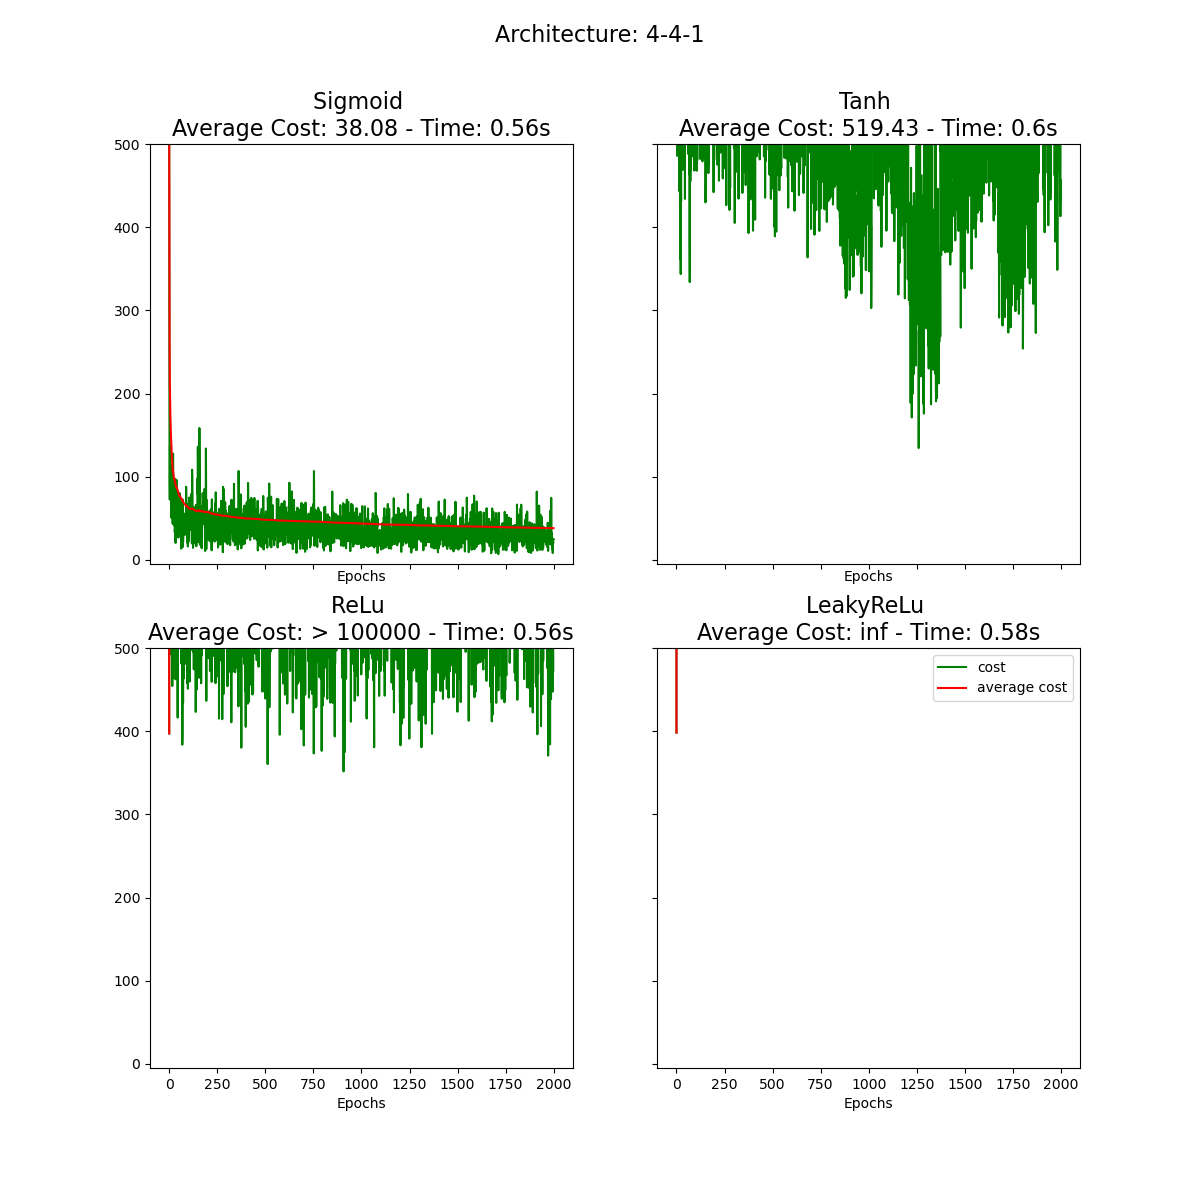
\includegraphics[scale=0.54]{MLP/Graphs/twoHidden.png}
\caption{Architecture Comparison 2}
\label{a42}
\end{figure}
\end{center}

\newpage
\subsection{Number of Neurons}
Contrary to the number of layers, the number of the neurons seem to help the algorithm converge. It is visible that the TanH activation function experienced an improvement compared to the test ran before which suggests that if the number of hidden layers are enough to grasps the complexity of the data, the number of neurons plays a more important role in the Neural Network's ability to achieve better results.

\begin{center}
\begin{figure}[htp]
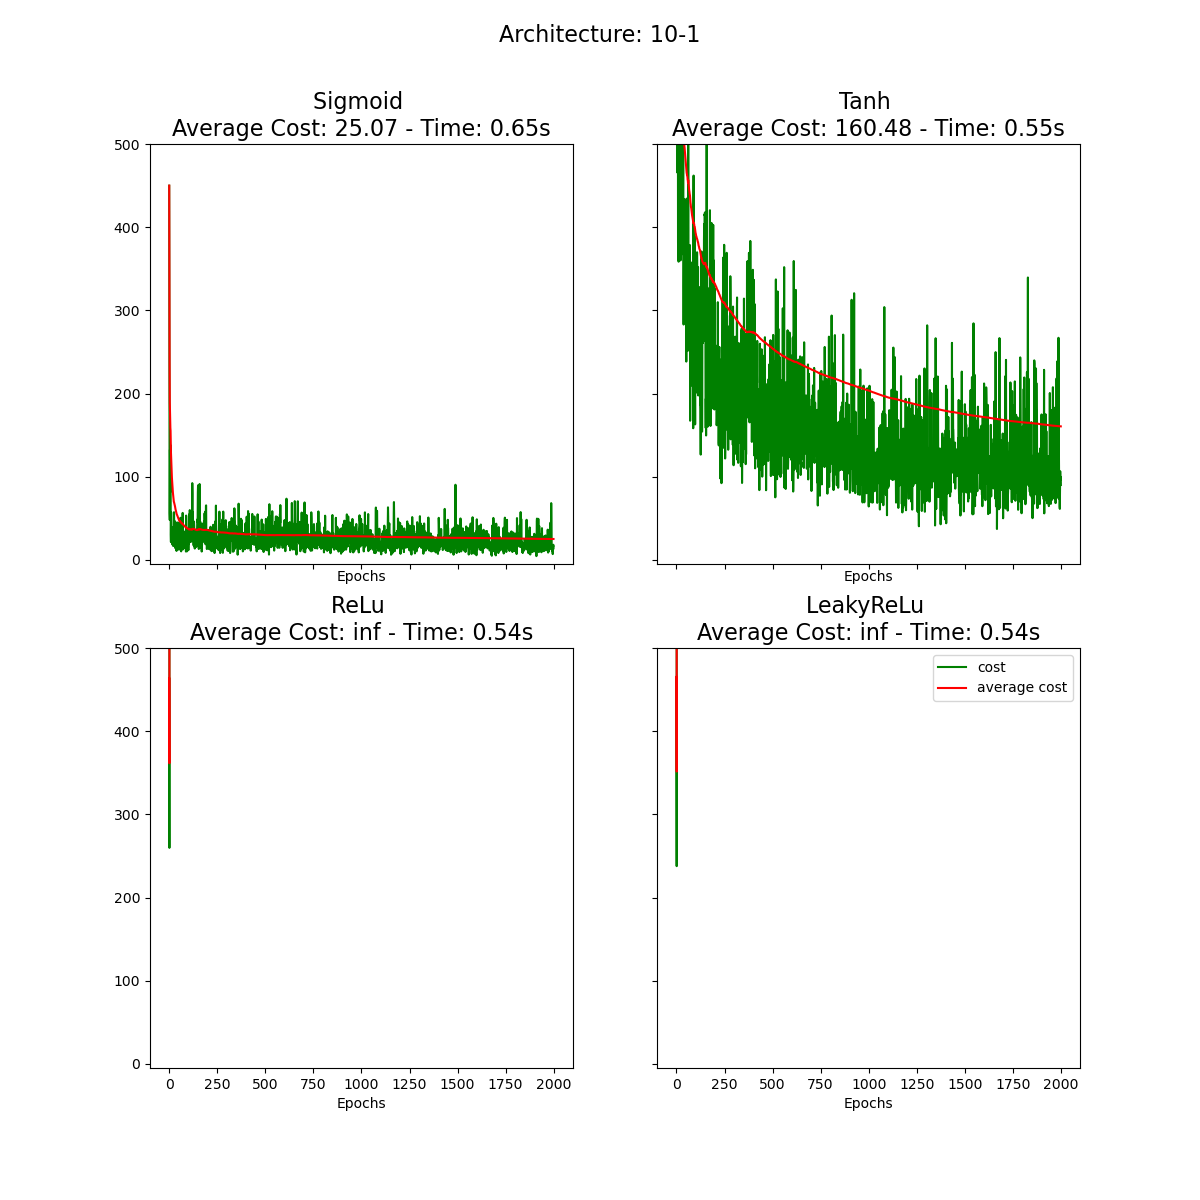
\includegraphics[scale=0.54]{MLP/Graphs/oneHiddenMoreN.png}
\caption{Neurons Comparison}
\label{n1}
\end{figure}
\end{center}

\subsection{Different Dataset}
The data bellow represents the \href{https://scikit-learn.org/stable/modules/generated/sklearn.datasets.load_diabetes.html#sklearn.datasets.load_diabetes}{diabetes dataset} and contains ten features bounded between $[-0.2,0.2]$ and the output is an integer contained in the interval $[25,346]$. The number of samples in the datasets are 442.

The training took place with the optimal parameters from the previous tests, that means that the learning rate assigned to ReLu, LeakyReLu and TanH is lower than the one assigned to Sigmoid, while the number of hidden layers in the Sigmoid and TanH was set lower than the ReLu ones.

From the graph below, it can be seen that the best cost achieved it was based on the TanH activation function while the Sigmoid scored the second. A reason why TanH outperformed Sigmoid might be given its ability to encode negative relationships. 


\begin{center}
\begin{figure}[htp]
\includegraphics[scale=0.54]{MLP/Graphs/diabetesComparison.png}
\caption{Diabetes Comparison}
\label{diabetes}
\end{figure}
\end{center}

\chapter{Evolutionary Optimisation}


\section{Genetic Algorithms}
The genetic algorithms are part of a family of algorithms that try to reproduce the Darwinian evolution through a simple representation of it. The main inherited principles are:
\begin{enumerate}
\item Variation - individuals differ from each other
\item Inheritance - traits are passed from a specimen to the other
\item Selection - the best adapted individual will be more successful at surviving
\end{enumerate}

In essence, the genetic algorithms implement those through the individual representation (the chromosome) and various genetic operators such as mutation and crossover. 

\subsection{Implementation}

First thing on the pipeline of a genetic algorithm is the individual representation. The chromosome is represented by a genotype that encodes the genes of the individual. Generally speaking, those can be represented in binary form, as integers or as real numbers. Whilst the algorithms architecture can be represented as binary numbers - such as if a neuron is used or not - in the specific case of weights representation, the only reasonable choice is the real number representation. As such, the first thing that needs to be set is the length of the chromosome. In order to automate the process of length selection, a function has been created which takes a model with its architecture, passes the data through it in order to initialises the weights and counts the parameters.

\lstinputlisting[language=Python, firstline=42, lastline=57]{Genetic/GA.py}

Once this is accomplished, the function returns the parameters - which contain the weights shape, the bias and the number of parameters for each layer - and the number of parameters in total which is used to initialise the individual. Before creating the individual, the fitness goal must be specified (maximising or minimising the goal) after which the individual can be created and it will take a representation of a list.

\lstinputlisting[language=Python, firstline=78, lastline=80]{Genetic/GA.py}

Next, it is required to specify the function that is needed to create the individual. Firstly, a function that returns a random float within specified boundaries is created:

\lstinputlisting[language=Python, firstline=82, lastline=83]{Genetic/GA.py}

which is then registered as a function that creates the floating attribute

\lstinputlisting[language=Python, firstline=86, lastline=87]{Genetic/GA.py}

followed by the creation of a function that generates individuals by repeating the previous function n times:
\lstinputlisting[language=Python, firstline=88, lastline=90]{Genetic/GA.py}

The population is created in a similar manner, by repeating the creation of individuals for n times.

\lstinputlisting[language=Python, firstline=92, lastline=93]{Genetic/GA.py}

The next step is to define the genetic operators. For this case, the selection operator chosen has been the Tournament Selection with a size of two.

\lstinputlisting[language=Python, firstline=144, lastline=145]{Genetic/GA.py}

The Crossover operator has been selected to be the Simulated Binary Crossover which guarantees that the average of the offspring values is the same as the parents one:

\lstinputlisting[language=Python, firstline=146, lastline=147]{Genetic/GA.py}

While the mutation operator has been selected to be the polynomial function.:

\lstinputlisting[language=Python, firstline=149, lastline=152]{Genetic/GA.py}

The evaluation function was implemented using the parameters information from the first function in order to recreate the network from the genotype and used the model in order to return the cost:

\lstinputlisting[language=Python, firstline=97, lastline=139]{Genetic/GA.py}

which has been passed to the evaluation function:

\lstinputlisting[language=Python, firstline=142, lastline=143]{Genetic/GA.py}

Now that the all the processes and representations are defined, the algorithm is able to start.

\lstinputlisting[language=Python, firstline=155, lastline=189]{Genetic/GA.py}


\newpage
\subsection{Results}

\subsubsection{Populations}

The first variable that is affected by the change in population, as visible from the graph, is the time. Whilst with a higher population comes a longer time, the algorithm doesn't seem to improve significantly.

\begin{center}
\begin{figure}[htp]
\includegraphics[scale=0.70]{Genetic/Graphs/GA/populationComparison.png}
\caption{Population Comparison}
\label{populations}
\end{figure}
\end{center}

\newpage
\subsubsection{Generations}
When observing the generation parameter, it is visible that it suffers from the same trade-off as the population. While a greater amount of generations managed to find a better solution, it took a significant amount of time. 

\begin{center}
\begin{figure}[htp]
\includegraphics[scale=0.70]{Genetic/Graphs/GA/generationsComparison.png}
\caption{Generations Comparison}
\label{generations}
\end{figure}
\end{center}

\newpage
\subsubsection{Mutation Probabilities}

Compared to the hyperparameters above, a higher mutation did not significantly affect the time although it affected the solution, resulting in the best solution being found with a lower mutation probability. It is visible from the graph that the population suffers great peaks, signalling that mutation diversifies the population but in the process, good individuals are lost. 

\begin{center}
\begin{figure}[htp]
\includegraphics[scale=0.70]{Genetic/Graphs/GA/mutationComparison.png}
\caption{Mutation Probability Comparison}
\label{mutation}
\end{figure}
\end{center}

\newpage
\subsubsection{Crossover Probabilities}

Contrary to Mutation, a higher probability of crossover positively affected the population, managing to find the best solution when the probability was equal to 60\%.

\begin{center}
\begin{figure}[htp]
\includegraphics[scale=0.70]{Genetic/Graphs/GA/crossoverComparison.png}
\caption{Crossover Probability Comparison}
\label{crossover}
\end{figure}
\end{center}



\newpage
\section{Particle Swarm Optimisation(PSO)}

The PSO algorithm imitates the behaviour of groups of organisms. This particles move in the sample space, looking for solutions and are are abiding simple rules.

Each iteration of the PSO algorithm updates the position of every particle and the solution gets evaluated. Both the best position of the swarm and of the individual particles are being tracked and are updated based on the inertia (speed and direction of movement).



\subsection{Implementation}
The encoding of the chromosome and the evaluation of the individual have remained the same as in the case of the Genetic Algorithm. The particle gets created by inheriting from the NumPy array and gets two different attributes, speed and best:

\lstinputlisting[language=Python, firstline=141, lastline=143]{Genetic/PSO.py}

The particle creator will create a random array within the specified boundaries, representing the position and the particle speed:

\lstinputlisting[language=Python, firstline=146, lastline=155]{Genetic/PSO.py}

The particle update rule is assigned to a function:


\lstinputlisting[language=Python, firstline=164, lastline=187]{Genetic/PSO.py}

The flow of the algorithm is implemented as following:

\lstinputlisting[language=Python, firstline=194, lastline=241]{Genetic/PSO.py}
\newpage
\subsection{Results}
\subsubsection{Swarm Size}
The size of the swarm seem to have a massive impact on the time whilst showing considerable improvements in the minimum cost. It can be seen that after a swarm size of 100, the swarm size slightly improved the result while considerable affecting the time variable.
\begin{figure}[htp]
\centering
\includegraphics[scale=0.70]{Genetic/Graphs/PSO/swarmSize.png}
\caption{Swarm Size Comparison}
\label{sizeSwarm}
\end{figure}

\newpage
\subsubsection{Generations}
The number of generations that pass until the algorithm finishes influences the result substantially as well as the time. Compared to the Swarm size, the effect of the generations on time has been much more tolerant, the algorithm being able to achieve a similar result in a much lower amount of time.
\begin{figure}[htp]
\centering
\includegraphics[scale=0.70]{Genetic/Graphs/PSO/swarmGenerations.png}
\caption{Swarm Generations Comparison}
\label{generationsSwarm}
\end{figure}


\chapter{Conclusion}

Considering all of the algorithms, the results seem to change between each problem, with no set of parameters being able to generalise to another problem. While in general they all found good solutions to the problems at hand, they all require time to converge to an optimal solution and they might overfit in the attempt to find one. The PSO and GA seemed to find a solution in more time than the gradient descent training method although they have the ability to work with functions that are not continuous, while the normal training method is bounded to use continuous activation functions.

\include{1}
%\include{code}
%\bibliographystyle{abbrv}
\bibliography{references}

\end{document}